\section{Extension}
In computer science, things are changing fast, which leads to a raise of obsolete results. Specially when it comes to Comparison studies,One can't cover all the candidates. 
Moreover, between the initial experiment and the published results there might be new candidates and an evolution of
others. Therefore we Propose new creterioin for a successful experiment ~Extension~.
In our content Extension means the ability to provide the necessary tools to not only Repeat the experiment but to be able to add extra candidates, Workloads or metrics.


\begin{figure}%[!htb]
    \center{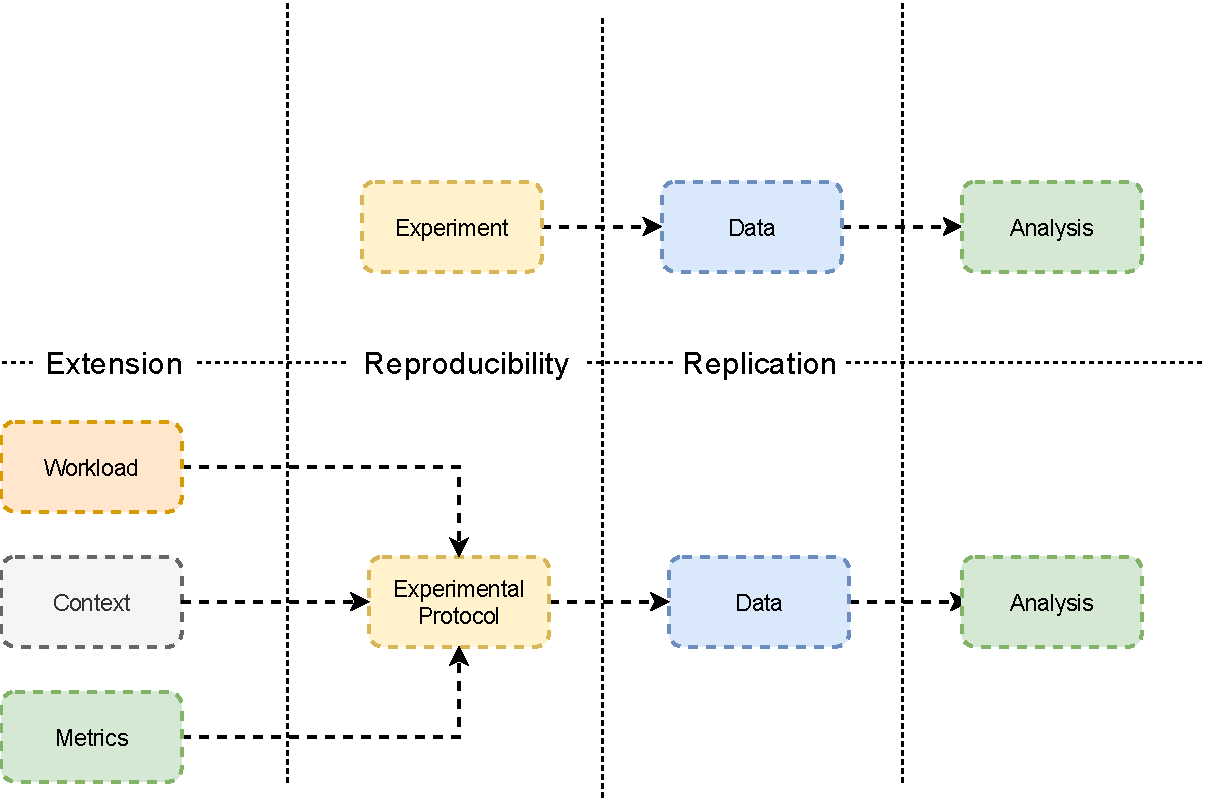
\includegraphics[width=.9\linewidth]{imgs/benchmarkingprotocol}}
    \caption{Benchmarking protocol}\label{fig:benchmarkingprotocol}
\end{figure}


\section{Perspectives}
By the end of this study we have gathered enought guidelines to make the tests more reproducible, accurate.
We created a set of new tests named \textbf{energy tests} which are more similar to performance tests. Thanks to the work of two interns [ mamadou and adrien] we created a CI/CD plateform to measure the energy consumption of Java projects and we could track the evolution of the this energy accross different stages of the project.
In the figure below we see an example of this plugin.
For more details please visit the gitlab repository ... add link.

\begin{figure}%[!htb]
    \center{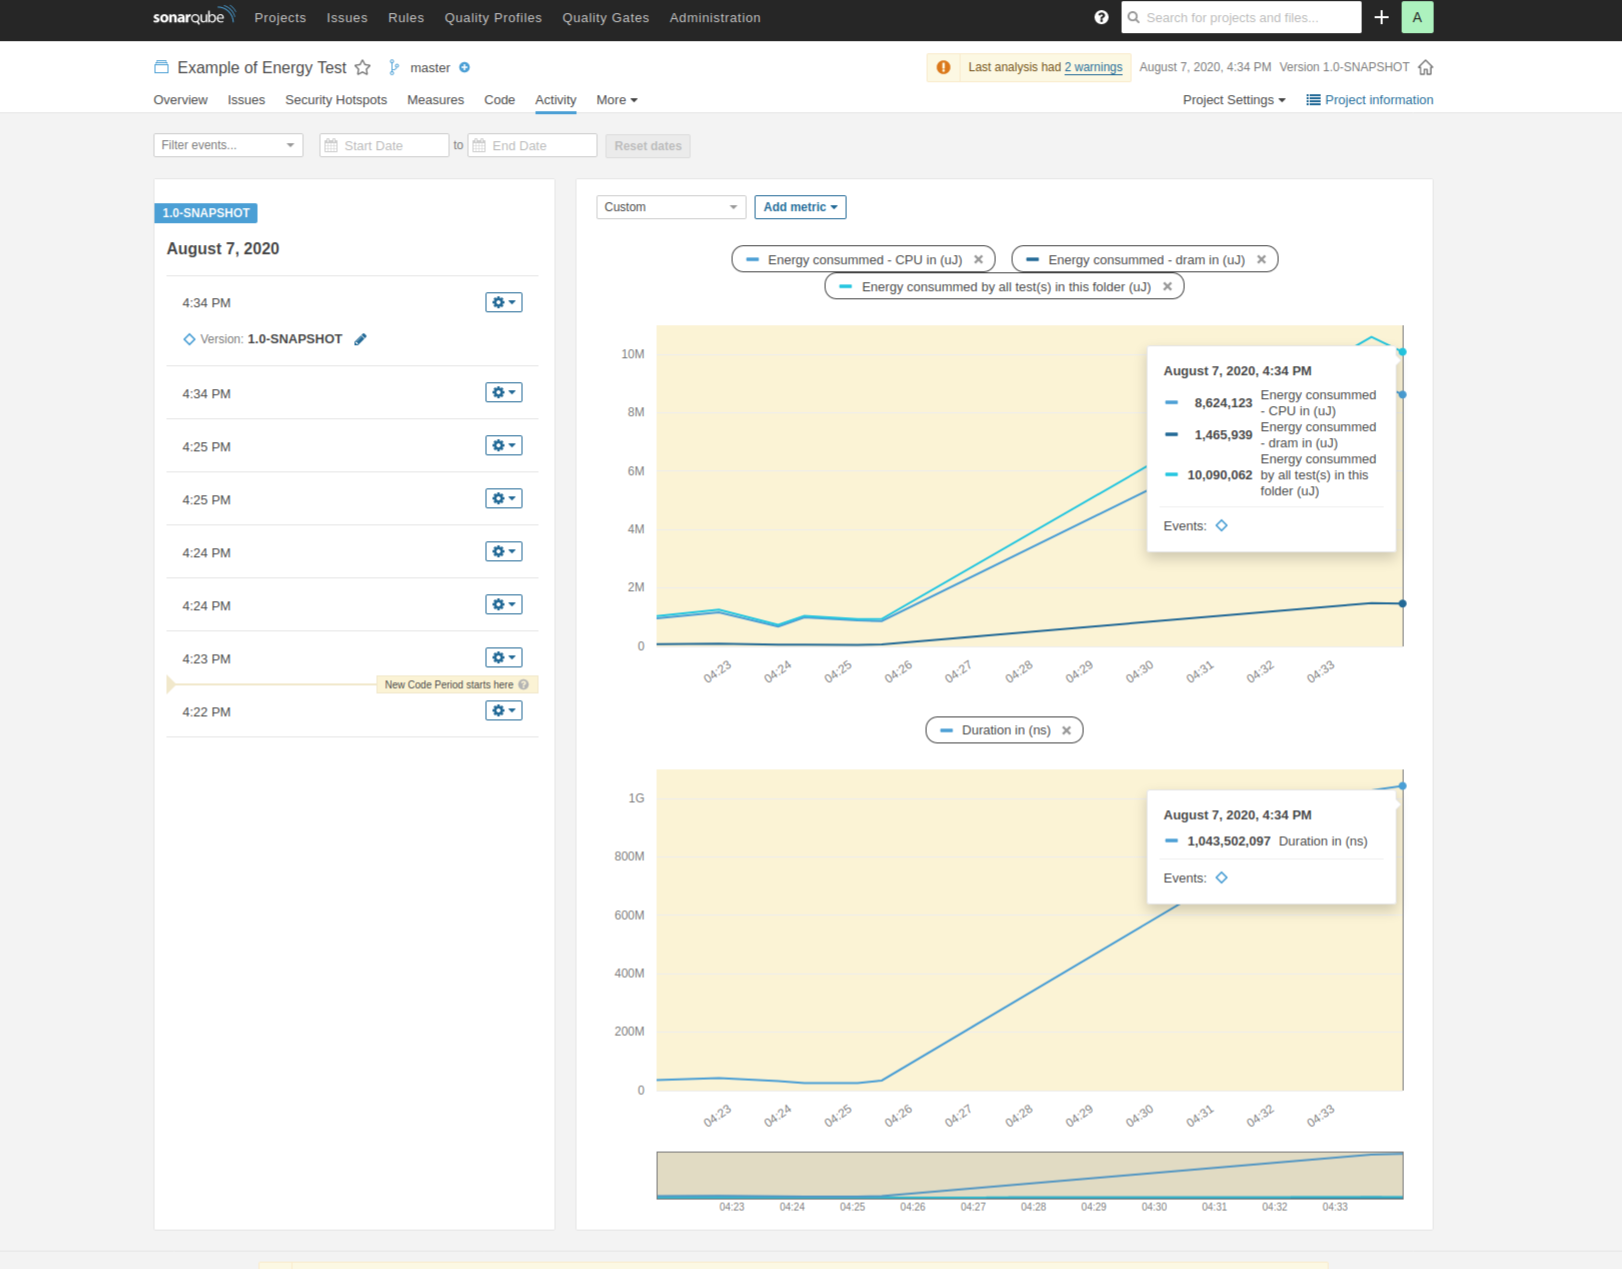
\includegraphics[width=.9\linewidth]{imgs/JunitSonarplugin}}
    \caption{Example of the Junit Sonar Plugin}\label{fig:sonar_plugin}
\end{figure}
